\icode{E-MC-SI-L2-261026-005}
一带电粒子（重力不计），在匀强电场\(E\)中从\(a\)运动到\(b\)的运动轨迹如图中虚线所示，电场方向竖直向下。若不计空气阻力，下列说法正确的是\paren[]

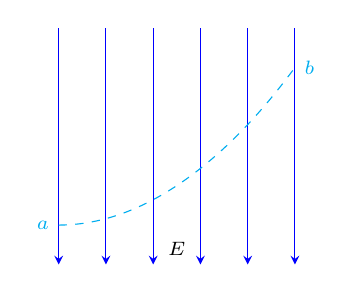
\begin{tikzpicture}[>=stealth,font=\scriptsize]
	\foreach \x in {0,.6,...,3.1}
		\draw[->,blue] (\x,0)--++(0,-3);
	\draw[dashed,cyan] (0,-2.5)node[left]{ \(a\)} parabola bend(0,-2.5)(3,-.5)node[right]{ \(b\)};
	\node at(1.5,-2.8){ \(E\)};
\end{tikzpicture}
\begin{choices}
	\item 粒子带正电
	\item \(a\)点电势高于\(b\)点
	\item 运动过程中粒子的动能减小
	\item 运动过程中粒子的电势能减小
\end{choices}
\begin{answer}
	D\qquad 提示：由轨迹判断出电场力竖直向上
\end{answer}